 \section{Klasyfikacje reprezentacji geometrii}
\label{sec:rep}
Wybór reprezentacji geometrycznej określa dopuszczalne operacje oraz strukturę danych przechowywanych w pamięci. Dzieli się na dwie główne kategorie: jawne (w tym parametryczne) oraz uwikłane \cite{botsch2010, piegl1997}.

Reprezentacje jawne i parametryczne definiują powierzchnię poprzez podanie współrzędnych punktów. Jawne stosują funkcję, która mapuje przestrzeń trójwymiarową na dwuwymiarową, a parametryczne opisują punkty powierzchni poprzez niezależne zmienne pomocnicze.

Modele uwikłane opisują powierzchnię jako zbiór punktów spełniających równanie $f(x,y,z) = 0$, gdzie funkcja zwraca wartość skalarną dla każdego punktu przestrzeni trójwymiarowej.

W niniejszej pracy omówiono trzy modele geometryczne. Siatki trójkątów i powierzchnie NURBS\footnote{Non-Uniform Rational Basis Splines} należą do reprezentacji parametrycznych. Natomiast funkcje odległości ze znakiem (SDF\footnote{Signed Distance Function}) przedstawiają podejście uwikłane.

Powodem wyboru siatek trójkątów, powierzchni NURBS oraz funkcji odległości ze znakiem jako obiekty mojej analizy, była chęć przedstawienia trzech fundamentalnych a jednocześnie różnych podejść reprezentacji geometrii. Każda z nich wspiera inny proces, czy to precyzyjne modelowanie inżynieryjnie czy modelowanie rzeźbiarskie. Zbadanie tych podejść pozwoli na analizę porównawczą metod reprezentacji geometrii trójwymiarowej.

Reprezentacje mają swoje zalety i wady, co wymusza wybór odpowiedniego rozwiązania dla danego problemu, czy wymagana jest precyzja krzywych, jakie operacje muszą być wspierane oraz jakie są ograniczenia obliczeniowe. Każde z tych zagadnień wpływa na decyzje o wyborze reprezentacji danych.

\subsection{Siatki trójkątów}
\label{sec:mesh}

\begin{figure}[h!]
    \centering
    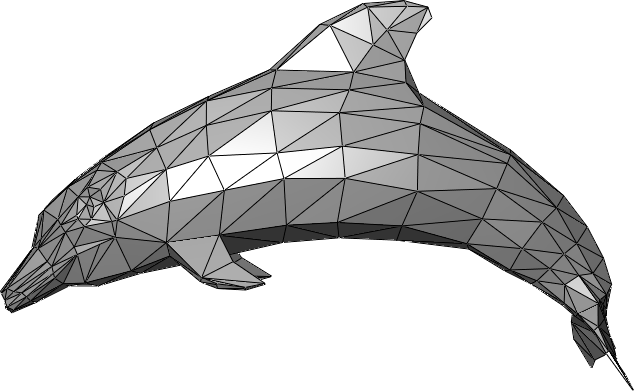
\includegraphics[width=\columnwidth]{media/Dolphin_triangle_mesh.png}
    \caption{Siatka modelu delfina. Chrschn, Public domain, via Wikimedia Commons}
    
\end{figure}

\paragraph{Definicja i historia}
Standard, który został przyjęty na kartach graficznych to siatki trójkątów. Trzy wierzchołki, które nie są współliniowe, wyznaczą dokładnie jedną płaszczyznę, co w wypadku czworokątów nie jest zawsze gwarantowane.

Siatka trójkątów jest zdefiniowana jako $M=(V,E,F)$, gdzie $V = \{v_1,...,v_{|V|}\}$ to zestaw wierzchołków, $E = \{e_1,...,e_{|E|}\}$ to krawędzie między wierzchołkami a $F = \{f_1,...,f_{|F|}\}$ to zestaw ścian. Każda ściana jest określona przez unikalną trójkę wierzchołków należących do zbioru $V$. W najprostszych strukturach krawędzie nie są przechowywane w pamięci, ale wynikają z definicji ścian.

Każdy z trójkątów w siatce posiada wektor normalny, który wyznacza się przez iloczyn wektorowy krawędzi:
\begin{equation}
    \mathbf{n} = (v_2 - v_1) \times (v_3 - v_1)
\end{equation}
Kierunek normalnej jest określony przez kolejność wierzchołków i pozwala określić orientację, co jest podstawą technik takich jak \textit{back-face culling}, który jest używany przez karty graficzne do odrzucania niewidocznych powierzchni w trakcie renderowania.

Dla zamkniętej siatki spełniającej warunek rozmaitości 2-wymiarowej zachodzi tożsamość Eulera:
\begin{equation}
    V - E + F = 2
\end{equation}
gdzie $V$ to liczby wierzchołków, $E$ krawędzi i $F$ ścian, spełnienie warunku jest wymagane przez większość algorytmów operujących na siatkach \cite{botsch2006}.

Przed przejściem do struktur danych warto wyjaśnić rozmaitość 2-wymiarową, jest to pojęcie z zakresu topologii, które pojawia się w literaturze dotyczącej reprezentacji geometrii trójwymiarowej. W kontekście siatek wielokątowych wymaga spełnienia dwóch warunków. Pierszy z nich to, że każda krawędź może należeć do maksymalnie dwóch trójkątów, a drugi mówi że otoczenie każdego wierzchołka musi tworzyć pojedyńczy wspólny wachlarz wielokątów. Krawędzie należące do dokładnie jednego trójkąta są definicją otworu, w przypadku siatek zamkniętych każda krawędź jest współdzielona przez dokładnie dwa trójkąty, co gwarantuje brak dziur \cite{bloom1997}.

\paragraph{Struktury danych}

Dobór struktury danych do przechowywania siatki wpływa na sprawność operacji lokalnych.

Najprostsza struktura to \textit{Indexed Face Set}, przechowująca listę wierzchołków oraz listę ścian jako trójki indeksów wierzchołków. Pozwala to na uniknięcie duplikowania współrzędnych wierzchołków współdzielonych przez sąsiednie trójkąty. Natomiast wadą jest brak możliwości efektywnego odpytania o sąsiedztwo. Aby wyznaczyć sąsiednie ściany danego wierzchołka wymogiem jest przeszukanie całej listy \cite{kettner1998}. 

W celach optymalizacji stosowane są rozszerzone struktury danych, które przetrzymują wskaźniki do sąsiednich elementów.

\textit{Winged-Edge Data Structure} przechowuje dla każdej krawędzi osiem referencji: wierzchołek początku i końca, lewą i prawą ścianę, oraz cztery sąsiednie krawędzie, tzw. "skrzydła" od których wynosi się nazwa struktury. Wadą takiego podejścia jest fakt, że krawędź nie posiada orientacji, przy przechodzeniu przez siatkę potrzebna jest weryfikacja kierunku ruchu \cite{kettner1998}.

\textit{Half-edge Data Structure} powstała jako rozwiązanie problemów obejmujących poprzednio omówioną strukturę. Polega na podzieleniu każdej krawędzi na dwie pół-krawędzie z przeciwnymi orientacjami, dzięki czemu zawsze znają własną stronę skierowania. Każda przechowuje wskaźniki do: wierzchołka do którego prowadzi, ściany po lewej stronie, następnej i przeciwnej pół-krawędzi, sprawia to że przechodzenie po siatce jest jednoznaczne. Podobnie jak Winged-Edge, struktura \textit{half-edge} modeluje orientowalne 2-rozmaitości, przy czym orientacja jest opisana bezpośrednio w pół-krawędziach \cite{kettner1998}.

Wybór struktury innej niż IFS ma wyraźny wpływ na wydajność narzędzi do edycji. Algorytmy jak wygładzanie czy podział powierzchni wymagają częstego odpytywania o sąsiedztwo wierzchołków i modyfikowania topologii. W strukturze IFS\footnote{Indexed Face Set} znalezienie sąsiednich ścian wymusza przeszukanie całej listy, co przy modelach mających miliony trójkątów daje złożoność $O(F)$. Struktura taka jak \textit{half-edge} redukuje tę operację do $O(1)$.

\paragraph{Zastosowania}
Siatki trójkątów są stosowane niemal wszędzie gdzie wymagana jest reprezentacja geometrii 3D, zarówno w zastosowaniach w czasie rzeczywistym jak i w renderowaniu offline.

W grach komputerowych każdy obiekt sceny reprezentowany jest przez siatkę, ponieważ karty graficzne posiadają dedykowany sprzęt do rasteryzacji trójkątów. W animacji filmowej, studia takie jak Pixar, czy DreamWorks wykorzystują siatki jako format modeli postaci i środowisk. Druk 3D wykorzystuje format STL, oparty o listę trójkątów spełniających warunek rozmaitości 2-wymiarowej.

\paragraph{Zalety i wady}
Główną zaletą siatek trójkątów jest uniwersalność oraz natywne wsparcie sprzętowe kart graficznych, co czyni je dominującą reprezentacją geometrii w grafice komputerowej. Prostota struktury umożliwia efektywną implementację szerokiego zakresu algorytmów. Wadą natomiast jest charakter aproksymacyjny reprezentacji, wierne odwzorowanie gładkich krzywych powierzchni wymaga bardzo gęstej siatki, która jest obliczeniowo droga, lub zastosowania powierzchni podziału, takich jak algorytm Catmull-Clark, który iteracyjnie wygładza siatkę przez dodawanie nowych wierzchołków \cite{halstead1993}.

\subsection{Powierzchnie NURBS}
\label{sec:nurbs}

\paragraph{Definicja i historia}
Przed komputerami inżynierowie opisywali krzywe za pomocą fizycznych splajnów, czyli elastycznych listw trzymanych obciążnikami. Matematycznym odpowiednikiem są wielomiany, jednak mają poważne ograniczenia: nie pozwalają na precyzyjny opis krzywych stożkowych, a ich współczynniki nie są intuicyjne z geometrycznego punktu widzenia \cite{rogers2001}.

Pierre Bézier zaproponował reprezentację, która jest oparta na punktach kontrolnych. Niestety jego metoda miała wadę, przy złożonych kształtach wymagała wielomianów wysokiego stopnia, które są niestabilne numerycznie \cite{rogers2001}.

Rozwiązaniem stały się krzywe B-splajnowe. Składają się z wielu połączonych fragmentów wielomianów niskiego stopnia, a zakres wpływu punktów kontrolnych jest ograniczony za pomocą tablicy węzłów. Chociaż B-splajny pozbyły się niestabilności numerycznej, wciąż opierały się na wielomianach, przez co nie pozwalały na dokładny opis krzywych stożkowych \cite{rogers2001, piegl1997}.

Krzywe NURBS rozwiązują ten problem poprzez wprowadzenie wag do punktów kontrolnych, odpowiada to matematycznemu dodaniu czwartej współrzędnej. Krzywa powstaje poprzez rzut z przestrzeni czterowymiarowej, umożliwia to dokładny opis krzywych stożkowych \cite{piegl1997}.

\begin{figure}[h!]
    \centering
    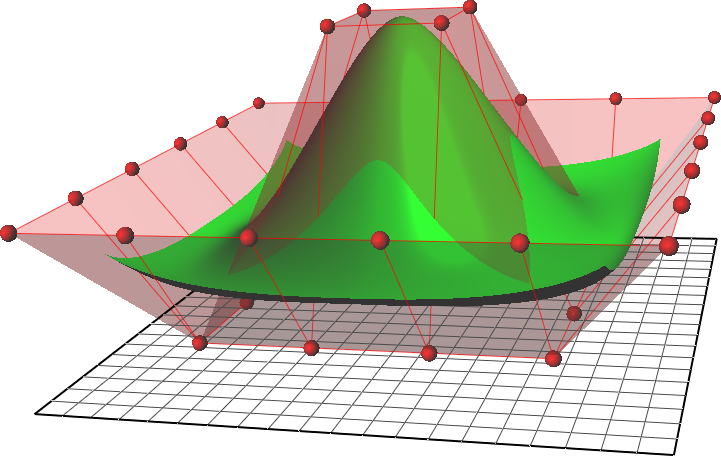
\includegraphics[width=\columnwidth]{media/NURBS_surface.png}
    \caption{Powierzchnia NURBS. Accountalive, CC BY-SA 3.0, via Wikimedia Commons}
    
\end{figure}

\paragraph{Zasada działania}
Krzywa NURBS o stopniu $d$ z punktami kontrolnymi $\mathbf{b}_0,\ldots, \mathbf{b}_n$, wagami $w_0,\ldots,w_n$ oraz tablicą węzłów $t_0,\ldots,t_m$ jest definiowana jako \cite{duncan2005}:
\begin{equation}
    \mathbf{B}(t) = \frac{\sum_{i=0}^{n} w_i \mathbf{b}_i N_{i,d}(t)}
    {\sum_{i=0}^{n} w_i N_{i,d}(t)}
\end{equation}
gdzie $N_{i,d}(t)$ to funkcje B-splajnu zdefiniowane na tablicy węzłów. Węzły $t_i$ są parametrami wyznaczającymi lokalizację funkcji, co oznacza, że każdy punkt kontrolny wpływa tylko na fragment odpowiadający jego przedziałowi, a nie na całą krzywą. 

Przekształcenia afiniczne stosuje się do krzywej NURBS poprzez zastosowanie ich na punkty kontrolne. Kształt krzywej można modyfikować przez zmianę pozycji punktów kontrolnych i przez zmianę ich wag, gdzie zwiększenie wagi przyciąga krzywą bliżej do danego punktu, jest to intuicyjnym rozwiązaniem. Krzywe NURBS są niezmienne zarówno przy przekształceniach afinicznych jak i rzucie perspektywicznym, co jest istotną właściwością dla zastosowań w grafice komputerowej \cite{piegl1997}.

\paragraph{Struktury danych}
Minimalna struktura danych, która opisuje krzywą NURBS zawiera: wielokąt kontrolny, który jest zestawem punktów kontrolnych wraz z wagami, stopień krzywej oraz tablice węzłów \cite{piegl1997}. Pełny zestaw danych obejmuje też najwyższe indeksy punktów kontrolnych i węzłów, jednak z perspektywy programisty działającego na gotowej krzywej wystarczy minimalna forma. W przypadku powierzchni NURBS struktura rozszerza się do siatki punktów kontrolnych $m \times n$, dwóch stopni oraz dwóch tablic węzłów.

\paragraph{Zastosowania}
Krzywe NURBS są stosowane głównie w miejscach gdzie jest wymagana precyzja opisu geometrii. Systemy CAD/CAM wykorzystują je jako podstawową reprezentację swoich krzywych i powierzchni, ponieważ dokładność jest tam konieczna, aby móc wytwarzać lub obrabiać części maszynowo. W przemysłach samochodowych i lotniczych NURBS umożliwia tworzenie powierzchni aerodynamicznych oraz przeprowadzanie akuratnych symulacji na modelach. Mimo dominacji siatek wielokątów w animacji i grach, każde profesjonalne oprogramowanie do modelowania trójwymiarowego obsługuje NURBS jako format.

\paragraph{Zalety i wady}
Główna zaleta krzywych NURBS to możliwość precyzyjnego opisu krzywych stożkowych takich jak okręgi czy elipsy, na co krzywe Béziera nie pozwalają. Modyfikacja kształtu dzięki węzłom, pozwala na edytowanie jedynie fragmentu krzywej bez przekształcania pozostałej części modelu. Następną zaletą jest fakt, że taka reprezentacja jest numerycznie stabilna w porównaniu do wielomianów wysokiego stopnia. 

Wadą natomiast jest nieintuicyjność punktów kontrolnych, ponieważ krzywa nie przechodzi przez te punkty, ale jest przez nie sterowana. Złożona topologia, jest trudna do ujęcia za pomocą krzywych NURBS. Pod względem implementacyjnym ta reprezentacja jest bardziej złożona niż siatki trójkątów \cite{piegl1997}.

Ważną przeszkodą powierzchni NURBS jest potrzeba na regularną siatkę punktów kontrolnych $m \times n$. Uniemożliwia ona swobodne modelowanie skomplikowanych obiektów, trudne modele potrzebują ręcznego łączenia wielu osobnych czworokątnych łat NURBS. Proces jest numerycznie niestabilny, co często prowadzi do powstawania dziur na złączach, jest to jedną z większych wad względem siatek wielokątnych.

\subsection{Funkcje odległości ze znakiem (SDF)}
\label{sec:sdf}

\paragraph{Definicja i historia}
Reprezentacja uwikłana opisuje powierzchnie jako zbiór punktów, które spełniają równanie $f(\mathbf{x}) = 0$. Zależnie od znaku zwróconej przez funkcję wartości jesteśmy w stanie określić względne położenie punktu od powierzchni. $f(\mathbf{x}) < 0$ oznacza wnętrze bryły, $f(\mathbf{x}) > 0$ oznacza że punkt jest na zewnątrz, natomiast $f(\mathbf{x}) = 0$ leży dokładnie na powierzchni \cite{osher2003}

Ta właściwość daje przewagę nad reprezentacjami jawnymi w sprawdzaniu przynależności punktu do obiektu. Modele jawne wymagają rzut promienia, który zlicza ilość przecięć z powierzchnią, parzysta liczba oznacza, że punkt jest na zewnątrz obiektu, a nieparzysta wewnątrz. W reprezentacji uwikłanej potrzeba jedynie obliczyć $f(\mathbf{x})$ i sprawdzić znak \cite{osher2003}.

\begin{figure}[h!]
    \centering
    \includesvg[width=\columnwidth]{media/SDF_duck.svg}
    \caption{Wizualizacja dyskretnego pola odległości ze znakiem w kształcie kaczki. Drummyfish, CC0, via Wikimedia Commons}
\end{figure}

\paragraph{Zasada działania}
Funkcja odległości ze znakiem jest przypadkiem reprezentacji uwikłanej, gdzie wartość funkcji zwraca odległość do najbliższej powierzchni i jest definiowana ogólnym wzorem:
\begin{equation}
    d(\mathbf{x}) = \min_{\mathbf{x'} \in \partial\Omega} 
    \|\mathbf{x} - \mathbf{x'}\|
\end{equation}
gdzie $\partial\Omega$ to powierzchnia obiektu. Gradient funkcji $\nabla d(\mathbf{x})$ jest wersorem, czyli wektorem jednostkowym i wskazuje kierunek najbliższego punktu na powierzchni \cite{osher2003}.

\begin{figure}[h!]
    \centering
    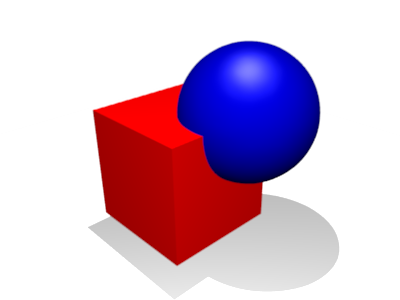
\includegraphics[width=0.32\columnwidth]{media/Boolean_union.png}\hfill
    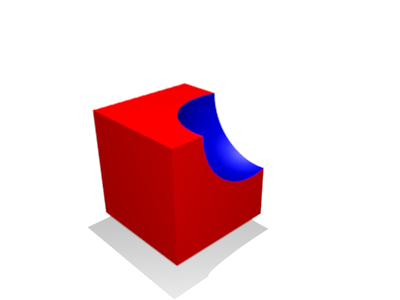
\includegraphics[width=0.32\columnwidth]{media/Boolean_difference.png}\hfill
    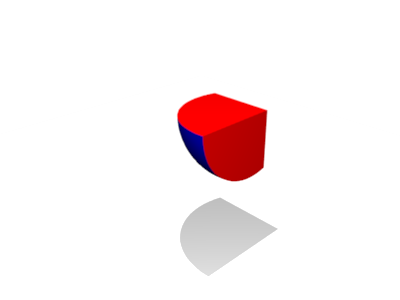
\includegraphics[width=0.32\columnwidth]{media/Boolean_intersect.png}
    
    \caption{Wyniki operacji boolowskich wykonanych na kostce i kuli: sumy, różnicy i części wspólnej}
\end{figure}


Reprezentacje uwikłane dają możliwość wykonywania operacji konstruktywnej geometrii brył CSG\footnote{Constructive Solid Geometry} przez proste operacje. Dla dwóch brył opisanych funkcjami $f_1$ i $f_2$ operacje Boola można zdefiniować jako:
\begin{align}
    f_1 \cup f_2 &= \min(f_1(\mathbf{x}),\ f_2(\mathbf{x})) \\
    f_1 \cap f_2 &= \max(f_1(\mathbf{x}),\ f_2(\mathbf{x})) \\
    f_1 \setminus f_2 &= \max(f_1(\mathbf{x}),\ -f_2(\mathbf{x}))
\end{align}

\paragraph{Struktury danych}
Najprostszą do zaimplementowania strukturą danych wykorzystywaną do przechowywania SDF jest gęsta siatka wokseli, gdzie woksel to najmniejszy element przestrzeni. Przestrzeń wokół obiektu jest dzielona na regularną trójwymiarową siatkę sześcianów, gdzie każdy woksel przechowuje jedną wartość zmiennoprzecinkową: odległość od najbliższej powierzchni. Taka struktura posiada dostęp do danych w czasie stałym $O(1)$ jako że jest stworzona z tablic, natomiast przynosi to też złożoność pamięciową rzędu $O(N^3)$, co wyklucza ją z użytkowania przy wysokich rozdzielczościach.

Zauważono właściwość, że wartości SDF bliskie zeru pojawiają się tylko w pobliży powierzchni, co doprowadziło do utworzenia metody wąskiego pasma \cite{sethian1999}. Technika polega na przechowywaniu precyzyjnych danych tylko w obszarze blisko powierzchni $f(\mathbf{x}) = 0$ i pomijaniu dalszych stref. Strukturą danych która odwzorowuje ten pomysł jest drzewo ósemkowe. Gdy dany obszar jest daleki od obiektu, to pozostaje niepodzielony jako liść drzewa. Przestrzeń która przecina powierzchnie jest rekurencyjnie dzielona na osiem sześcianów, do momentu osiągnięcia żądanej rozdzielczości. W reprezentacji drzewa korzeniem jest cała przestrzeń, a liście to obszary nie wymagające podziału.

\begin{figure}[h!]
    \centering
    \includesvg[width=\columnwidth]{media/Octree2.svg}
    \caption{Struktura drzewa ósemkowego. WhiteTimberwolf, CC BY-SA 3.0, via Wikimedia Commons}
\end{figure}

\paragraph{Zastosowania}
Funkcje odległości ze znakiem mają szerokie zastosowanie w grafice komputerowe i symulacjach fizycznych. Technika \textit{ray marching} używa SDF do adaptacji długości kroku wzdłuż promienia bez ryzykowania ominięcia powierzchni co przyśpiesza obliczenia w porównaniu do klasycznego \textit{ray castingu} \cite{hart1996}. SDF umożliwia też wydajne obliczanie miękkich cieni i okluzji, ponieważ odległość od powierzchni jest wbudowana w metodę. W symulacjach SDF jest wykorzystywany do detekcji i obsługi kolizji, szczególnie w symulacjach cieczy lub tkanin. Metoda cieszy się popularnością w robotyce.

\paragraph{Zalety i wady}
Główną zaletą SDF jest zwięzłość reprezentacji, powierzchnia jest w tej metodzie zdefiniowana analitycznie lub jako gęste pole wartości. Kolejną istotną zaletą jest możliwość wykorzystywania operacji takich jak CSG, czy trywialne obliczanie normalnych za pomocą gradientu. Jest to główna metoda wykorzystywana do algorytmów detekcji i kolizji, dzięki dostępowi do informacji w czasie stałym.

Wadą SDF są jej struktury danych, gdzie dla siatki wokseli złożoność pamięciowa wynosi $O(N^3)$. Struktury adaptacyjne takie jak drzewa ósemkowe ograniczają ten problem, ale kosztem złożoności czasowej i lokalności danych dla pamięci podręcznej procesora.

Ważnym ograniczeniem jest koszt jaki potrzeba podjąć przy aktualizacji danych. Dla obiektów dynamicznych konieczne jest przeliczenie pola odległości, co dla algorytmu \textit{Fast Sweeping Method} wynosi $O(N^3)$, a dla algorytmu \textit{Fast Marching Method} $O(N^3 \log N)$ \cite{sethian1999}. Sprawia to że SDF są trudne do stosowania w sytuacjach, gdy występuje częsta zmiana geometrii.

\subsection{Wnioski}
\label{sec:wnioski}

Każda z opisanych metod reprezentacji geometrii trójwymiarowej, siatki wielokątów, krzywe NURBS i reprezentacje oparte na funkcjach odległości ze znakiem posiadają swoje wady i zalety, które są wynikiem ich podstaw matematycznych. 

Wybór jednej z metod nad drugą nie powinien być kwestią preferencji, ale wynikać z analizy ograniczeń podanego problemu. Limity mogą być o charakterze obliczeniowym, takim jak budżet pamięci i czas albo geometrycznym, gdzie kształt musi mieć dokładną reprezentację charakterystycznej powierzchni, albo nawet narzucony format przez wymagane narzędzia. W praktyce to właśnie ograniczenia, a nie zalety mają rolę filtra, szybciej wyeliminują metody niż zalety wskażą optymalną metodę. Dopiero po zawężeniu listy możliwych rozwiązań, można zacząć porównywać różnice w wydajności i charakterze metod.

Pierwszym kryterium porównania jest swoboda topologiczna, czyli w jakim stopniu struktura reprezentacji ogranicza możliwości opisu obiektu. Siatki nie narzucają żadnych ograniczeń i pozwalają na złożone topologie. NURBS natomiast jest ograniczony ze względu na swoją definicję matematyczną, przez co skomplikowane topologię wymagają wykorzystania wielu łatek, między którymi pojawia się potrzeba zarządzania złączami, aby móc utworzyć reprezentację modelu. Funkcje odległości ze znakiem z kolei najlepiej z opisanych metod obsługują dynamiczne zmiany topologii, dzięki możliwości wykorzystywania operacji boolowskich i scalaniu powierzchni. Ograniczenie tej reprezentacji natomiast pojawia się podczas ekstrakcji danej geometrii, algorytmy wykorzystywane na tej metodzie mogą wprowadzać artefakty.

Precyzja w kontekście reprezentacji geometrii oznacza dokładność odwzorowania matematycznego modelu, względem otrzymanego kształtu obiektu, oraz ciągłość powierzchni opisaną klasami C0, C1 i C2. Siatki wielokątów gwarantują ciągłość C0, czyli przejście tylko między krawędzią styczności dwóch powierzchni, gdzie wciąż występuje ostre załamanie. Normalne są nieciągłe na krawędziach, natomiast dokładność wzrasta wraz z zagęszczeniem siatki. Reprezentacja NURBS jest dokładna ze względu na nature swojego opisu matematycznego, krzywe i powierzchnie są wyrażone analitycznie, co sprawia że ciągłość C2 - druga pochodna jest ciągła na złączeniu. Dzięki tym zależnością krzywe NURBS dominują w projektowaniu przemysłowym. SDF są analitycznie dokładne, natomiast po dyskretyzacji precyzja jest ograniczona poprzez rozdzielczość siatki wokseli. Gradient umożliwia dokładne kalkulację wektorów normalnych, ale tylko w miejscach gdzie pole odległości jest właściwie zdefiniowane. Spośród trzech omówionych metod NURBS jest jedyną która nie opiera się na przybliżeniach.

